\documentclass[tikz,border=8pt]{standalone}
\usepackage{amsmath,amssymb}
\usepackage[utf8]{inputenc}
\usepackage{tikz}
\usetikzlibrary{backgrounds,arrows.meta}

\tikzset{every picture/.style={line width=0.75pt}}

\definecolor{tensorblue}{rgb}{0.141,0.686,0.914}
\definecolor{matorange}{rgb}{0.937,0.620,0.039}
\definecolor{regionfill}{rgb}{0.420,0.267,0.267}

%% Grid: 4 cols x 4 rows, spacing S=80pt, tensor half-size H=11pt
%% Tensor (col c, row r) at (c*S, -r*S),  c,r in {0,1,2,3}
%% Subregion: cols {1,2}, rows {1,2}  (0-indexed)
%%
%% Bond labelling convention:  A^{col+1,row+1}  (1-indexed, col first = paper convention)

\begin{document}
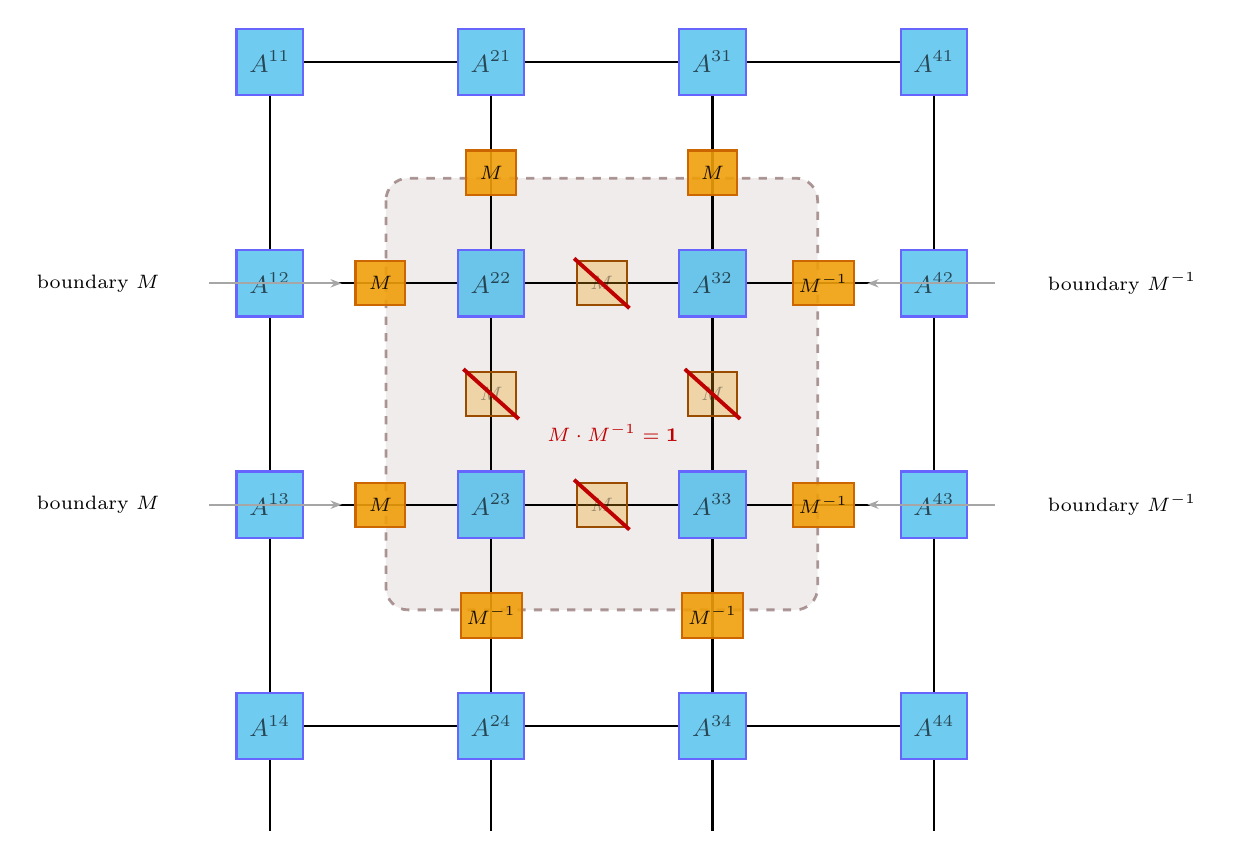
\begin{tikzpicture}[
    x=1pt, y=1pt,
    tensor/.style={
        rectangle, draw=blue!60, fill=tensorblue, fill opacity=0.65,
        inner sep=0pt, minimum width=24pt, minimum height=24pt, font=\small
    },
    mmat/.style={
        rectangle, draw=orange!80!black, fill=matorange, fill opacity=0.90,
        inner sep=1pt, minimum width=18pt, minimum height=16pt,
        font=\scriptsize\bfseries
    },
    minv/.style={
        rectangle, draw=orange!80!black, fill=matorange, fill opacity=0.90,
        inner sep=1pt, minimum width=22pt, minimum height=16pt,
        font=\scriptsize\bfseries
    },
    mcanc/.style={   % cancelled (interior) M
        rectangle, draw=orange!60!black, fill=matorange, fill opacity=0.30,
        inner sep=1pt, minimum width=18pt, minimum height=16pt,
        font=\scriptsize\bfseries, text opacity=0.35
    },
]

\def\S{80}   % grid spacing
\def\H{12}   % tensor half-width (bond starts H pt from centre)
\def\BL{26}  % extra bond length beyond grid edge (dangling legs)

%% ===================== BONDS (draw first, under tensors) =====================

%% Horizontal bonds
\foreach \c in {0,1,2} {
  \foreach \r in {0,1,2,3} {
    \pgfmathsetmacro{\xa}{\c*\S+\H}
    \pgfmathsetmacro{\xb}{(\c+1)*\S-\H}
    \pgfmathsetmacro{\y}{-\r*\S}
    \draw (\xa,\y) -- (\xb,\y);
  }
}

%% Vertical bonds
\foreach \c in {0,1,2,3} {
  \foreach \r in {0,1,2} {
    \pgfmathsetmacro{\x}{\c*\S}
    \pgfmathsetmacro{\ya}{-\r*\S-\H}
    \pgfmathsetmacro{\yb}{-(\r+1)*\S+\H}
    \draw (\x,\ya) -- (\x,\yb);
  }
}

%% Dangling (physical) legs — downward from each tensor
\foreach \c in {0,1,2,3} {
  \foreach \r in {0,1,2,3} {
    \pgfmathsetmacro{\x}{\c*\S}
    \pgfmathsetmacro{\ytop}{-\r*\S-\H}
    \pgfmathsetmacro{\ybot}{-\r*\S-\H-\BL}
    \draw (\x,\ytop) -- (\x,\ybot);
  }
}

%% ===================== SUBREGION shading =====================
\begin{scope}[on background layer]
  \fill[regionfill, opacity=0.10, rounded corners=8pt]
    (1*\S-38, -1*\S+38) rectangle (2*\S+38, -2*\S-38);
\end{scope}
\draw[regionfill, opacity=0.55, dashed, rounded corners=8pt, line width=1pt]
  (1*\S-38, -1*\S+38) rectangle (2*\S+38, -2*\S-38);

%% ===================== TENSORS =====================
%% Label: A^{col+1, row+1}  (1-indexed, matching paper: column index first)
\foreach \c/\cl in {0/1, 1/2, 2/3, 3/4} {
  \foreach \r/\rl in {0/1, 1/2, 2/3, 3/4} {
    \pgfmathsetmacro{\cx}{\c*\S}
    \pgfmathsetmacro{\cy}{-\r*\S}
    \node[tensor] (A\c\r) at (\cx,\cy)
      {$A^{\cl\rl}$};
  }
}

%% ===================== M INSERTIONS =====================
%%
%% Convention: applying M to the SUBREGION {col 1,2 ; row 1,2}
%% inserts M on every bond with at least one endpoint in the subregion.
%% Bonds entirely inside cancel (M * M^{-1} = 1); boundary bonds survive.
%%
%% Subregion tensors (0-indexed): (1,1),(2,1),(1,2),(2,2)
%%
%% --- Boundary bonds (survive) ---
%%
%%   Horizontal left   : col0-col1,  rows 1,2   => M on bond midpoint
%%   Horizontal right  : col2-col3,  rows 1,2   => M^{-1} on bond midpoint
%%   Vertical top      : row0-row1,  cols 1,2   => M on bond midpoint
%%   Vertical bottom   : row2-row3,  cols 1,2   => M^{-1} on bond midpoint

% Left boundary  (M)
\node[mmat] at (0.5*\S, -1*\S) {$M$};
\node[mmat] at (0.5*\S, -2*\S) {$M$};

% Right boundary (M^{-1})
\node[minv] at (2.5*\S, -1*\S) {$M^{-1}$};
\node[minv] at (2.5*\S, -2*\S) {$M^{-1}$};

% Top boundary (M)
\node[mmat] at (1*\S, -0.5*\S) {$M$};
\node[mmat] at (2*\S, -0.5*\S) {$M$};

% Bottom boundary (M^{-1})
\node[minv] at (1*\S, -2.5*\S) {$M^{-1}$};
\node[minv] at (2*\S, -2.5*\S) {$M^{-1}$};

%% --- Interior bonds (cancel) ---
%%
%%   Horizontal interior: col1-col2, rows 1 and 2
%%   Vertical interior:   row1-row2, cols 1 and 2

% Interior horizontal row 1  (col1-col2) — explicit coords: (120,-80)
\node[mcanc] (Mh1) at (120, -80) {$M$};
\draw[red!75!black, line width=1.4pt]
  (110, -71) -- (130, -89);

% Interior horizontal row 2  (col1-col2)  -- ALSO cancel M^{-1} from right side
\node[mcanc] (Mh2) at (1.5*\S, -2*\S) {$M$};
\draw[red!75!black, line width=1.4pt]
  (1.5*\S-10, -2*\S+9) -- (1.5*\S+10, -2*\S-9);

% Interior vertical col 1   (row1-row2)
\node[mcanc] (Mv1) at (1*\S, -1.5*\S) {$M$};
\draw[red!75!black, line width=1.4pt]
  (1*\S-10, -1.5*\S+9) -- (1*\S+10, -1.5*\S-9);

% Interior vertical col 2   (row1-row2)
\node[mcanc] (Mv2) at (2*\S, -1.5*\S) {$M$};
\draw[red!75!black, line width=1.4pt]
  (2*\S-10, -1.5*\S+9) -- (2*\S+10, -1.5*\S-9);

%% ===================== ANNOTATION =====================

%% Cancellation label — placed in empty space top-right inside region
\node[font=\scriptsize, text=red!75!black, align=center]
  at (1.5*\S+4, -1.5*\S-14) {$M \cdot M^{-1} = \mathbf{1}$};

%% Boundary labels: simple arrows from outside the grid to each boundary M box
%% Left boundary M's (at x=0.5*S, y=-1*S and y=-2*S)
\node[font=\scriptsize, align=right, text=black]
  at (-62, -1*\S) {boundary $M$};
\draw[-{Stealth[length=4pt]}, gray!70, shorten >=3pt]
  (-22, -1*\S) -- (0.5*\S-11, -1*\S);

\node[font=\scriptsize, align=right, text=black]
  at (-62, -2*\S) {boundary $M$};
\draw[-{Stealth[length=4pt]}, gray!70, shorten >=3pt]
  (-22, -2*\S) -- (0.5*\S-11, -2*\S);

%% Right boundary M^{-1}'s
\node[font=\scriptsize, align=left, text=black]
  at (3*\S+68, -1*\S) {boundary $M^{-1}$};
\draw[-{Stealth[length=4pt]}, gray!70, shorten >=3pt]
  (3*\S+22, -1*\S) -- (2.5*\S+13, -1*\S);

\node[font=\scriptsize, align=left, text=black]
  at (3*\S+68, -2*\S) {boundary $M^{-1}$};
\draw[-{Stealth[length=4pt]}, gray!70, shorten >=3pt]
  (3*\S+22, -2*\S) -- (2.5*\S+13, -2*\S);

\end{tikzpicture}
\end{document}
